\input{"C:/Users/spileggi/Google Drive/STAT 330/Lectures/SlideStyle.tex"}



\title[Lecture 11]{PROC TTEST, PROC CORR, Output Delivery System}
\author[Pileggi]{Shannon Pileggi}

\institute[STAT 330]{STAT 330}

\date{}


\begin{document}

\begin{frame}
\titlepage
\end{frame}

\begin{frame}
\frametitle{OUTLINE\qquad\qquad\qquad} \tableofcontents[hideallsubsections]
\end{frame}



%===========================================================================================================================
\section[The data]{Data}
%===========================================================================================================================
\subsection{}
%\begin{frame}
%\tableofcontents[currentsection, hideallsubsections]
%\end{frame}

\begin{frame}
\frametitle{Beat the Blues data}
\begin{itemize}
    \item
    enrolled patients with depression/anxiety
    \item
    randomly assigned them to Treatment as Usual (TAU) or BtheB, a new treatment delivery therapy via computers
    \item
    measured depression via Beck Depression Inventory (BDI) at baseline (pre-treatment), and 2, 4, 6, and 8 month follow up
    \item
    BDI scores range from 0 to 63 with higher scores indicating more severe depression
\end{itemize}
\end{frame}


%\begin{frame}[fragile]
%\frametitle{Get to know the data}
%\bmp{1.0\textwidth}
%\footnotesize
%\begin{code}{.0}
%libname flash "C:/Users/spileggi/Google Drive/STAT330/Data";
%
%proc contents data=flash.BtheB varnum; run;
%
%proc freq data=flash.BtheB; run;
%
%proc print data=flash.BtheB (obs=10); run;
%\end{code}
%\emp
%\end{frame}

\begin{frame}[fragile]
\frametitle{First 6 observations}
\bmp{1.05\textwidth}
\footnotesize
\begin{craw}{.0}{SAS output}
Obs  drug length treatment bdi\_pre  bdi\_2m bdi\_4m bdi\_6m  bdi\_8m
  1    No    >6m       TAU      29      2      2      .      .
  2   Yes    >6m     BtheB      32     16     24     17     20
  3   Yes    <6m       TAU      25     20      .      .      .
  4    No    >6m     BtheB      21     17     16     10      9
  5   Yes    >6m     BtheB      26     23      .      .      .
  6   Yes    <6m     BtheB       7      0      0      0      0
\end{craw}
\emp
\end{frame}

\begin{frame}
\frametitle{Review}
\oyo Match the appropriate statistical method for each research question.
\vskip10pt
\bmp{0.35\textwidth}
\be
\item one-sample t-test
\item two sample t-test
\item paired t-test
\item correlation
\ee
\emp
\bmp{0.10\textwidth} \hspace{0.05in} \emp
\bmp{0.55\textwidth}
\begin{enumerate}[]
\item[\underline{\hspace{0.25in}}] Is there a strong linear relationship between \ttt{bdi\_pre} and \ttt{bdi\_2m}?
\item[\underline{\hspace{0.25in}}] Does the population average of \ttt{bdi\_pre} differ from 20?
\item[\underline{\hspace{0.25in}}] On average in the population, does \ttt{bdi} change between the \ttt{pre} and \ttt{2m} measurements?
\item[\underline{\hspace{0.25in}}] Does population average \ttt{bdi} differ by whether or not patients were on anti-depressants (\ttt{drug})?
\end{enumerate}
\emp
\end{frame}

%===========================================================================================================================
\section[PROC TTEST]{PROC TTEST}
%===========================================================================================================================
\subsection{}
\begin{frame}
\tableofcontents[currentsection, hideallsubsections]
\end{frame}

\begin{frame}
\ft{Overview of PROC TTEST}
\bi
\item One sample t-test
\item Paired t-test (use \ttt{PAIRED} statement)
\item Two sample t-test (use \ttt{CLASS} statement)
\item[]
\item Options include
\bi
\item \ttt{H0 =} \emph{null value}
\item \ttt{ALPHA =} \emph{significance level}
\item \ttt{SIDES =} \ttt{U} \emph{(upper)}
    \item[] \hspace{0.44in} \ttt{L} \emph{(lower)}
    \item[] \hspace{0.44in} \ttt{2}  \emph{(two-sided)}
\ei
\ei
\end{frame}

\begin{frame}[fragile]
\ft{One sample t-test}
Does the population average baseline depression score differ from 20, at $\alpha=0.05$?  Test $H_0$: $\mu=20$ vs  $H_A$:  $\mu \neq 20$ \\
\vskip10pt
\bmp{1.0\textwidth}
\footnotesize
\begin{code}{.0}
PROC TTEST DATA = flash.BtheB H0 = 20 ALPHA = 0.05 SIDES = 2;
    VAR bdi_pre ;
RUN ;
\end{code}
\emp
\vskip10pt
Default settings are \fbox{\ttt{ALPHA = 0.05}} and \ttt{\fbox{SIDES = 2}}, so the only thing you must specify for this test is the null value of 20.
\end{frame}


\begin{frame}[fragile]
\ft{One sample t-test output}
\bmp{0.6\textwidth}
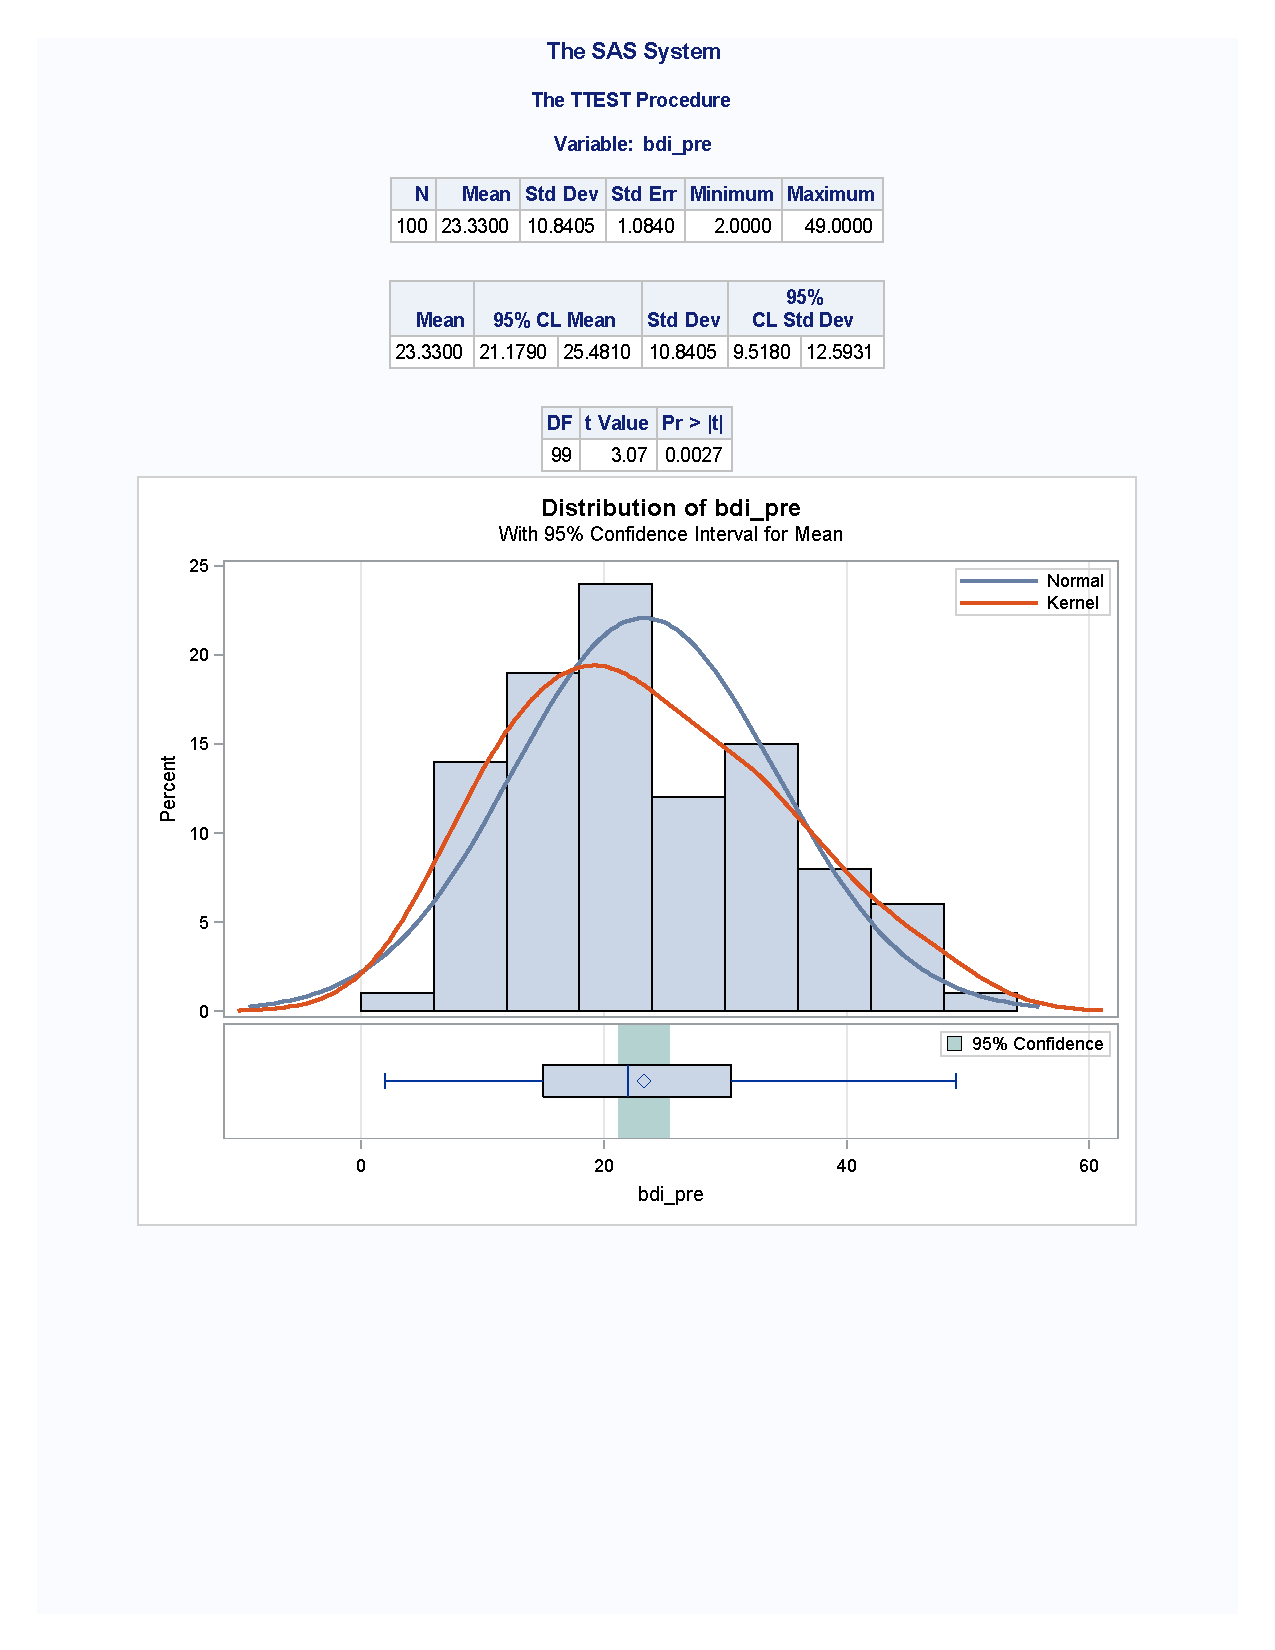
\includegraphics[trim=6.5cm 19.7cm 6.5cm 1.5cm,clip,width=1.0\textwidth]{L11_onesamplet.pdf}
\emp
\bmp{0.05\textwidth} \hspace{1in} \emp
\bmp{0.35\textwidth}
\begin{clicker}{We \underline{(do/do not)} have evidence that the \underline{(population/sample)} mean baseline BDI score differs from 20.}
\begin{enumerate}
\item do; population
\item do; sample
\item do not; population
\item do not; sample
\end{enumerate}
\end{clicker}
\emp
\end{frame}


\begin{frame}[fragile]
\ft{Two sample t-test}
Does the population average baseline depression score differ among patients who were and were not on antidepressants (\ttt{drug}), at $\alpha=0.05$?  Test $H_0$: $\mu_1=\mu_2$ vs  $H_A$:  $\mu_1 \neq \mu_2$ \\
\vskip10pt
\bmp{1.0\textwidth}
\footnotesize
\begin{code}{.0}
PROC TTEST DATA = flash.BtheB ALPHA = 0.05 SIDES = 2 ;
   VAR bdi_pre ;
   CLASS drug ;
RUN ;
\end{code}
\emp
\vskip10pt
Default settings are $H_0$: $\mu_1=\mu_2$, \fbox{\ttt{ALPHA = 0.05}}, and \ttt{\fbox{SIDES = 2}}, .
\end{frame}


\begin{frame}[fragile]
\ft{Two sample t-test output}
\bmp{0.6\textwidth}
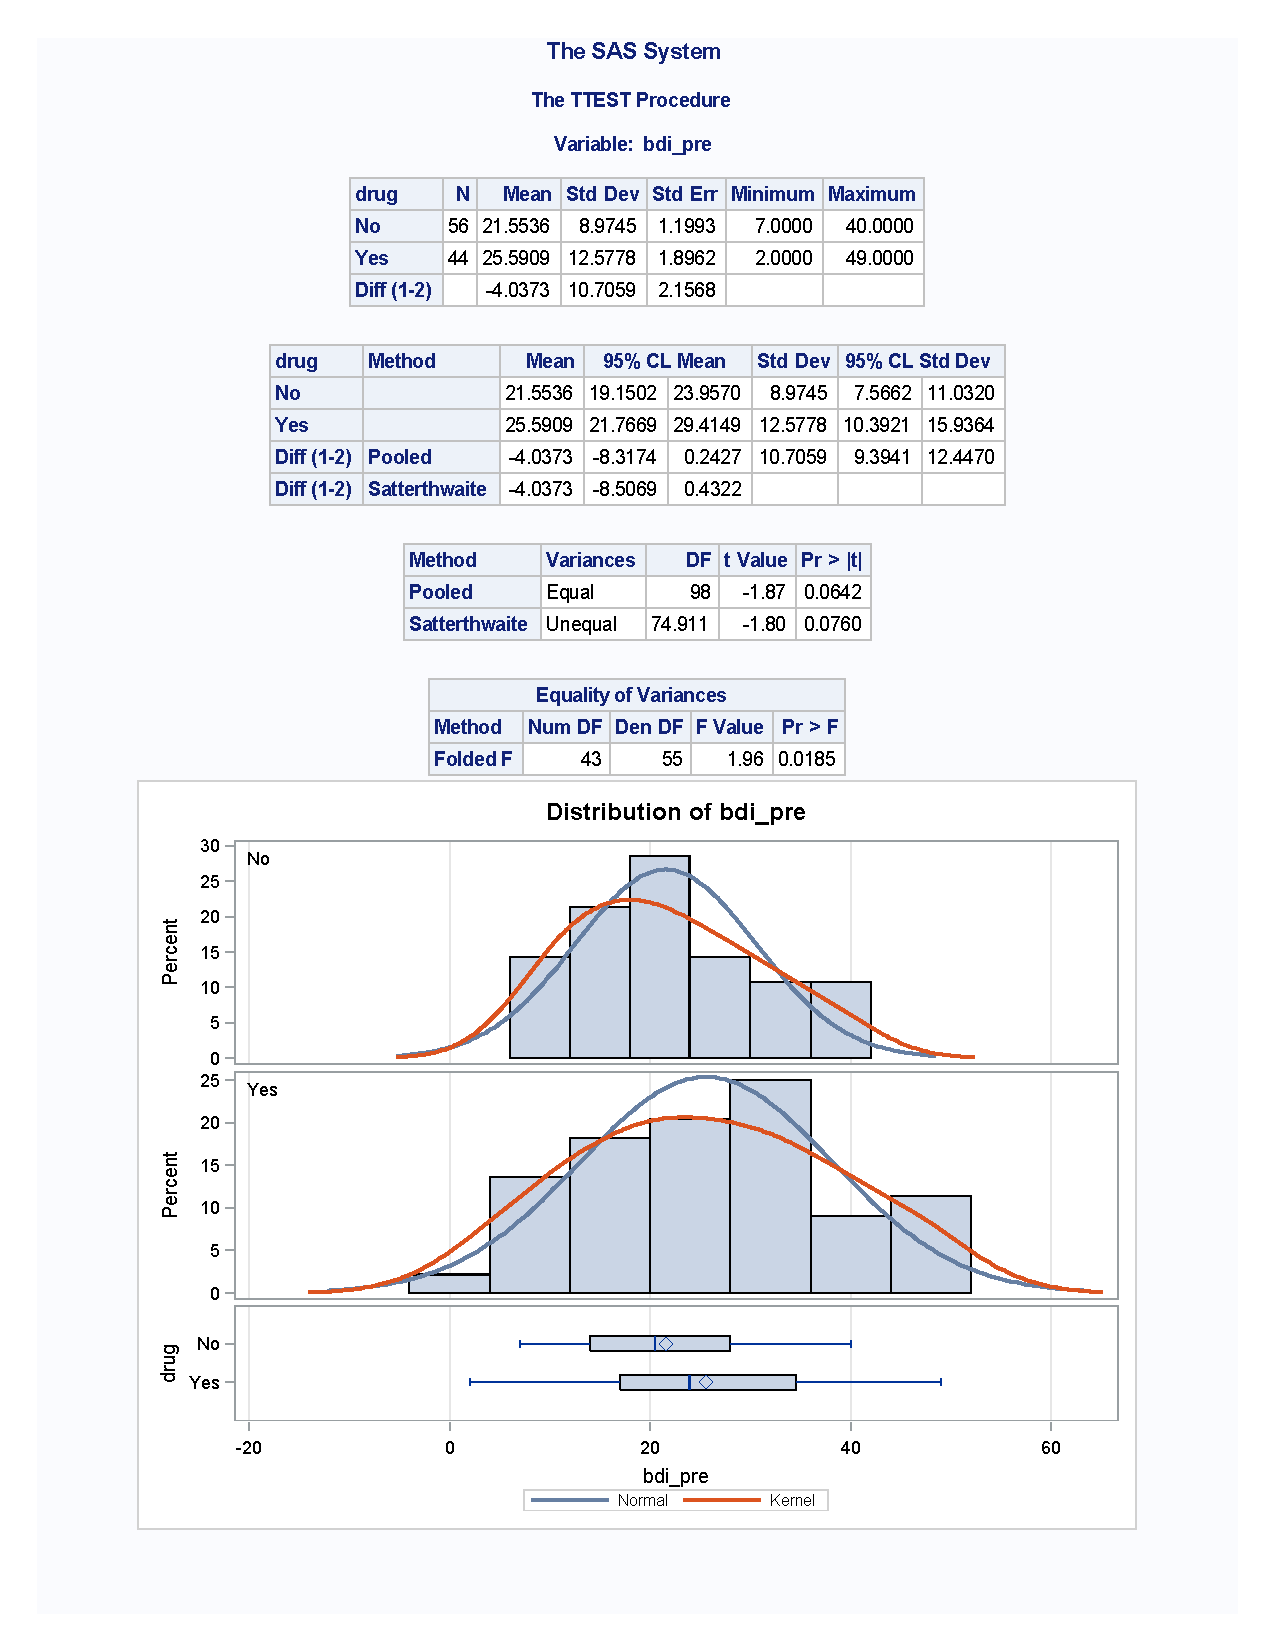
\includegraphics[trim=4.5cm 14.5cm 4.5cm 1.5cm,clip,width=1.0\textwidth]{L11_twosamplet.pdf}
\emp
\bmp{0.05\textwidth} \hspace{1in} \emp
\bmp{0.35\textwidth}
\begin{clicker}{We \underline{(do/do not)} have evidence that the population mean baseline BDI differs among the two groups.}
\begin{enumerate}
\item do
\item do not
\end{enumerate}
\end{clicker}
\emp
\end{frame}
%
%\begin{frame}[fragile]
%\ft{Two sample t-test select output}
%\bmp{1.05\textwidth}
%\footnotesize
%\begin{craw}{.0}{SAS output}
% drug          Method               Mean       95\% CL Mean
%
% No                              -------     -------  -------
% Yes                             -------     -------  -------
% Diff (1-2)    Pooled            -4.0373     -8.3174   0.2427
% Diff (1-2)    Satterthwaite     -4.0373     -8.5069   0.4322
%\end{craw}
%\emp
%\begin{clicker}{Which group has higher average baseline depression score?}
%\begin{enumerate}
%\item the \ttt{No} group
%\item the \ttt{Yes} group
%\end{enumerate}
%\end{clicker}
%\end{frame}

\begin{frame}[fragile]
\ft{Paired t-test}
Does the population average baseline depression score change between baseline and two month follow-up, at $\alpha=0.05$?  Let $\mu_d=\mu_{pre} -\mu_{2m}$; test $H_0$: $\mu_d=0$ vs  $H_A$:  $\mu_d \neq 0$ \\
\vskip10pt
\bmp{1.0\textwidth}
\footnotesize
\begin{code}{.0}
PROC TTEST DATA = flash.BtheB H0 = 0 ALPHA = 0.05 SIDES = 2 ;
   PAIRED bdi_pre*bdi_2m ;
RUN ;
\end{code}
\emp
\vskip10pt
Default settings are \fbox{\ttt{H0=0}}, \fbox{\ttt{ALPHA = 0.05}}, and \ttt{\fbox{SIDES = 2}}, so these options do not need to be specified.
\vskip10pt
For the paired t-test, you \ttb{cannot} use \fbox{\ttt{CLASS}} or \fbox{\ttt{VAR}} statements.
\end{frame}

\begin{frame}[fragile]
\ft{Paired t-test output}
\bmp{0.6\textwidth}
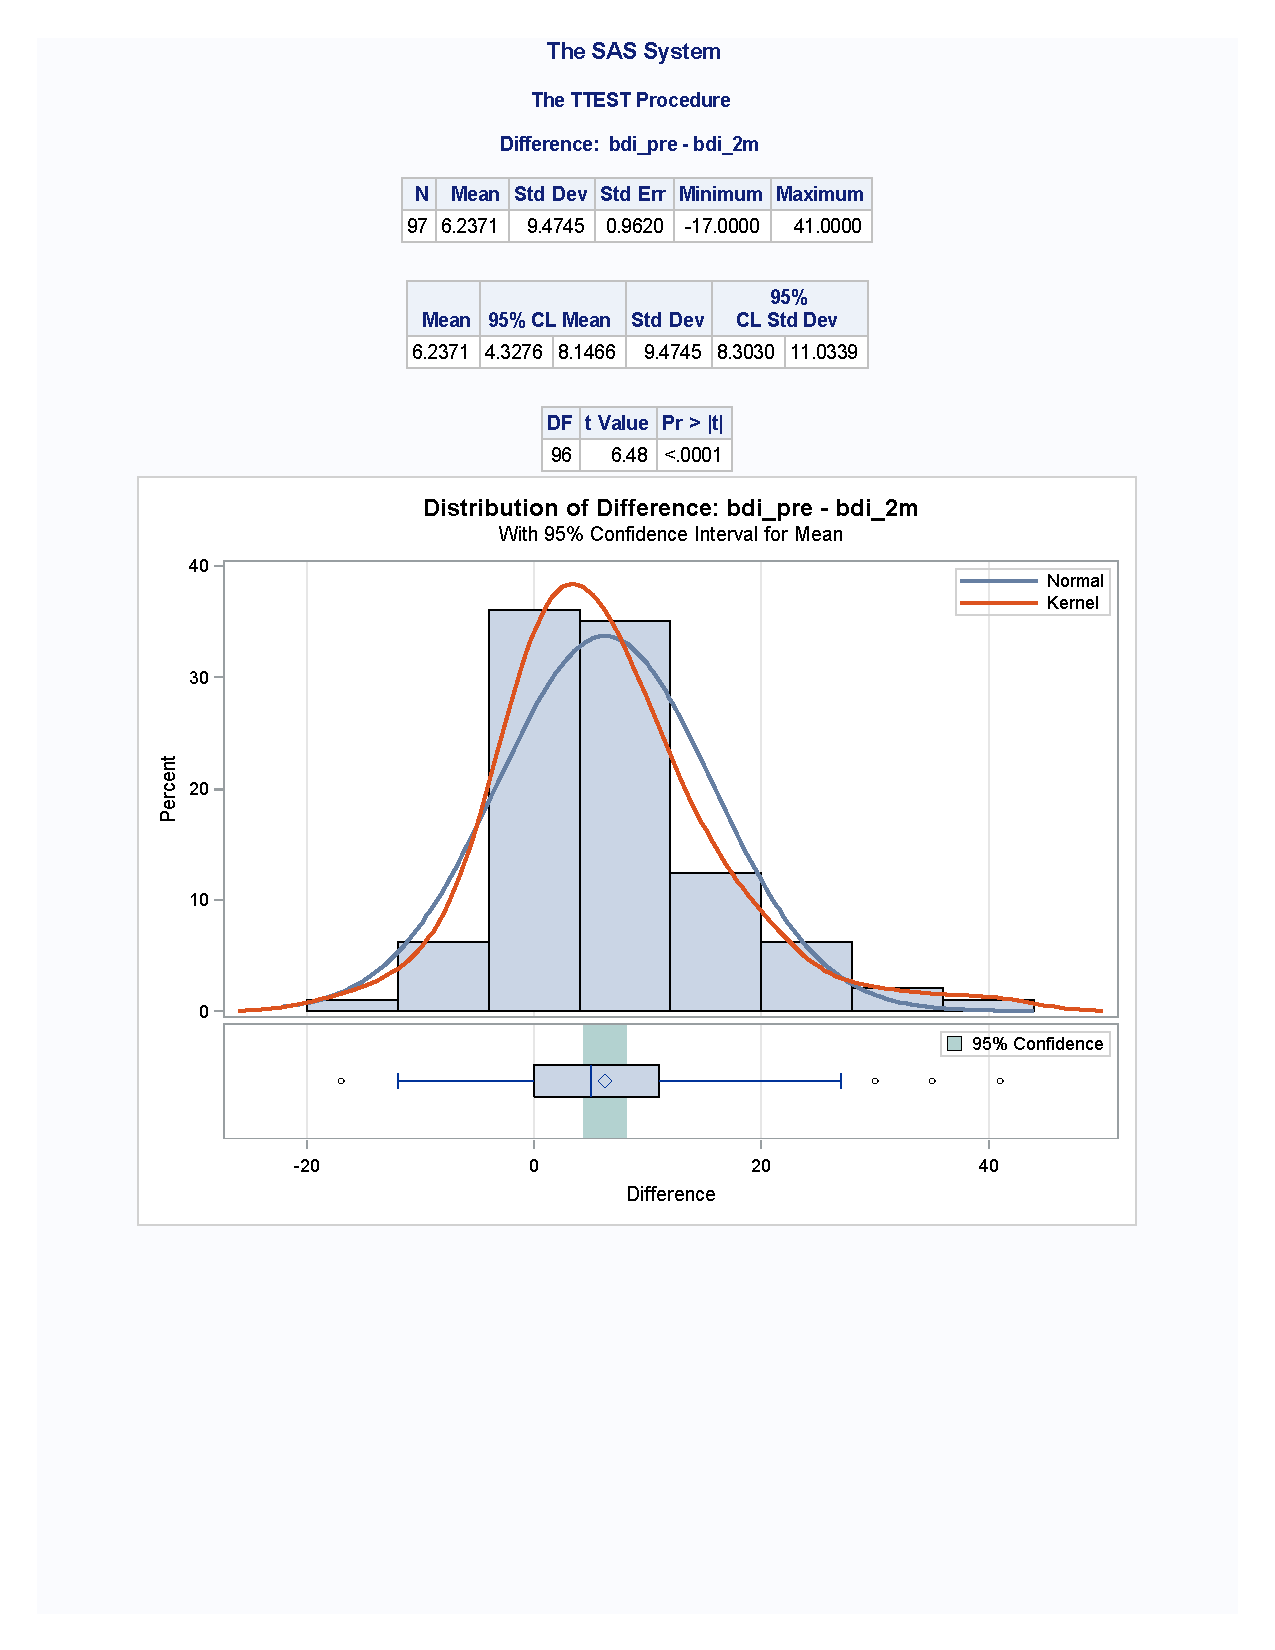
\includegraphics[trim=6.5cm 19.7cm 6.5cm 1.5cm,clip,width=1.0\textwidth]{L11_pairedt.pdf}
\emp
\bmp{0.05\textwidth} \hspace{1in} \emp
\bmp{0.35\textwidth}
\begin{clicker}{We \underline{(do/do not)} have evidence that the population mean BDI changes between baseline and 2 month follow up.  Furthermore, we have evidence that $\mu_{pre}$ is \underline{(greater/less)} than $\mu_{2m}$.}
\begin{enumerate}
\item do; greater
\item do; less
\item do not; greater
\item do not; less
\end{enumerate}
\end{clicker}
\emp
\end{frame}


%\begin{frame}[fragile]
%\ft{Paired t-test select output}
%\bmp{1.05\textwidth}
%\footnotesize
%\begin{craw}{.0}{SAS output}
%               Difference:  bdi_pre - bdi_2m
%
% N        Mean     Std Dev     Std Err     Minimum     Maximum
%
%97      6.2371      9.4745      0.9620    -17.0000     41.0000
%
%     Mean       95\% CL Mean        Std Dev      95\% CL Std Dev
%
%   6.2371      4.3276   8.1466      9.4745      8.3030  11.0339
%
%                   DF    t Value    Pr > |t|
%
%                   96       6.48      <.0001
%\end{craw}
%\emp
%\begin{clicker}{Which is larger?}
%\begin{enumerate}
%\bmp{0.2\textwidth} \item $\mu_{pre}$ \emp
%\bmp{0.2\textwidth} \item $\mu_{2m}$ \emp
%\end{enumerate}
%\end{clicker}
%\end{frame}



%\begin{frame}[fragile]
%\ft{Plots with PROC TTEST}
%\bmp{1.0\textwidth}
%\footnotesize
%\begin{code}{.0}
%ods graphics on;
%*example code from one sample t-test;
%proc ttest data=flash.BtheB H0=20  \underline{plots=all};
%	var bdi_pre;
%run;
%ods graphics off;
%\end{code}
%\emp
%\bi
%\item[]
%\item with any t-test you can request additional plots
%\item you will need to submit \fbox{\ttt{ods graphics on;}} to continue viewing/producing plots during your SAS session
%\ei
%\end{frame}


\begin{frame}
\ft{Checking conditions}
In general, conditions required for a t-test include:
\begin{enumerate}
\item Independent observations
\item Normal underlying distribution \emph{OR} $n>30$ (in each group for the two sample case)
\end{enumerate}
\vskip10pt
\oyo How would you go about checking these conditions in SAS?  What procedures/options would you use?
\end{frame}



%===========================================================================================================================
\section[PROC CORR]{PROC CORR}
%===========================================================================================================================
\subsection{}
\begin{frame}
\tableofcontents[currentsection, hideallsubsections]
\end{frame}

\begin{frame}
\ft{Overview of PROC CORR}
\bi
\item PROC CORR calculates Pearson's correlation coefficient by default
\bi
\item measures the strength of the linear relationship between two quantitative variables
\ei
\item To obtain Spearman's Rank Correlation use \fbox{\ttt{\footnotesize{PROC CORR SPEARMAN}}}
\bi
\item measures monotonic relationships between two variables (does not require linear relationship)
\ei
\item Use the \ttt{VAR} and \ttt{WITH} statements to specify the variables for computing the correlation matrix:
	\bi
	\item \ttt{VAR} variables are listed across columns
	\item \ttt{WITH} variables are listed along rows
    \item If \ttt{WITH} variables are omitted, then \ttt{VAR} variables are listed on both columns and rows - produces redundant information.
\ei
\ei
\end{frame}


\begin{frame}[fragile]
\ft{Correlation}
What is the strength of the linear relationship between baseline BDI and the follow-up BDI measurements?
\vskip10pt
\bmp{1.0\textwidth}
\footnotesize
\begin{code}{.0}
PROC CORR DATA = flash.BtheB ;
   VAR bdi_pre ;
   WITH bdi_2m bdi_4m bdi_6m bdi_8m ;
RUN ;
\end{code}
\emp
\end{frame}

\begin{frame}[fragile]
\ft{Correlation select output}
\bmp{0.50\textwidth}
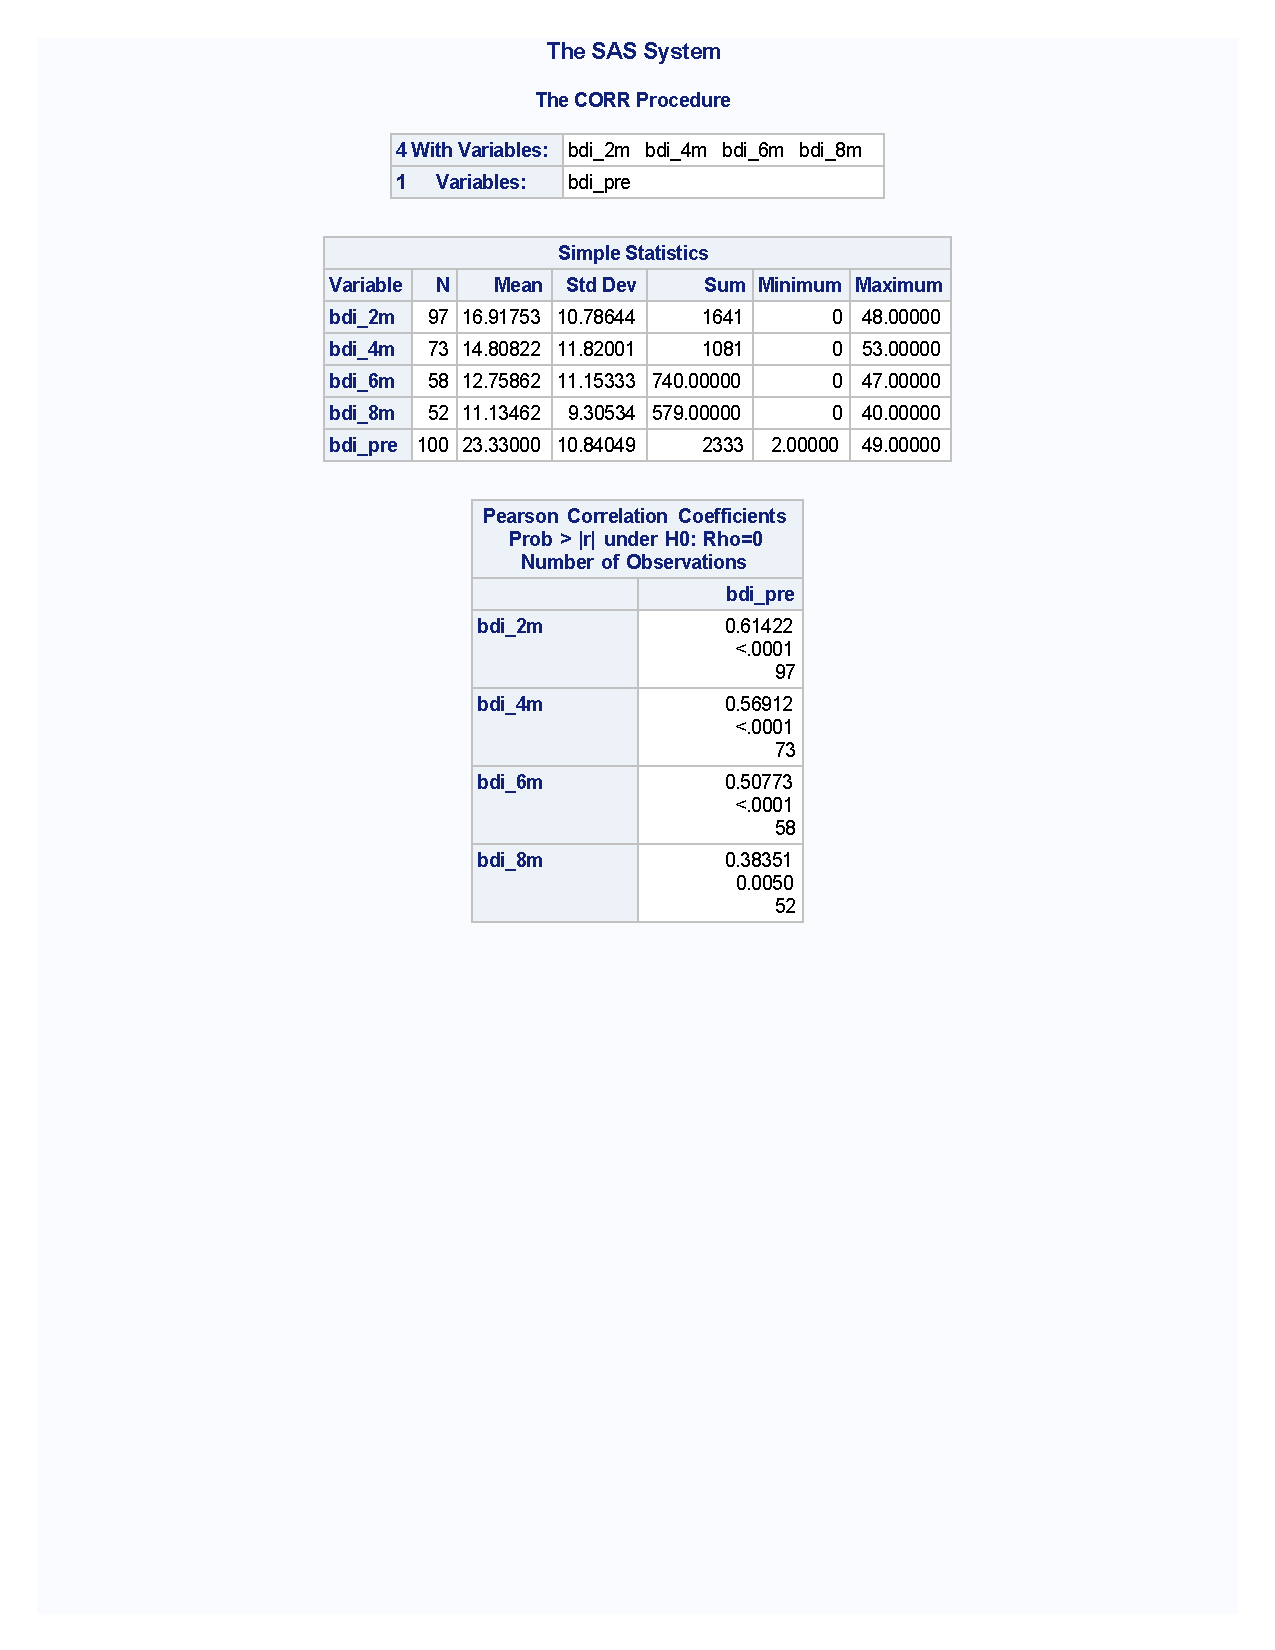
\includegraphics[trim=7.5cm 11cm 7.5cm 8cm,clip,width=1.0\textwidth]{L11_corr.pdf}
\emp
\bmp{0.05\textwidth} \hspace{0.05in} \emp
\bmp{0.50\textwidth}
The p-value tests\\ $H_0$: $\rho=0$ vs $H_A$: $\rho\neq0$.\\
\vskip5pt
\oyo
\begin{enumerate}
\item How important do you think the p-value is here?
\item Is the correlation between baseline BDI and follow-up measurements increasing or decreasing over time?
\item Why does $n$ change?
\end{enumerate}
\emp
\end{frame}

\begin{frame}[fragile]
\ft{Producing plots with PROC CORR}
How do you determine if Pearson's correlation is appropriate?
\vskip10pt
\hspace*{-0.2in}
\bmp{0.75\textwidth}
\footnotesize
\begin{code}{.0}
PROC CORR DATA = flash.BtheB \textcolor{OrangeRed}{PLOTS = matrix} ;
   VAR bdi_pre ;
   WITH bdi_2m bdi_4m bdi_6m bdi_8m ;
RUN ;
\end{code}
\emp
\bmp{0.10\textwidth} \hspace{1in} \emp
\bmp{0.25\textwidth}
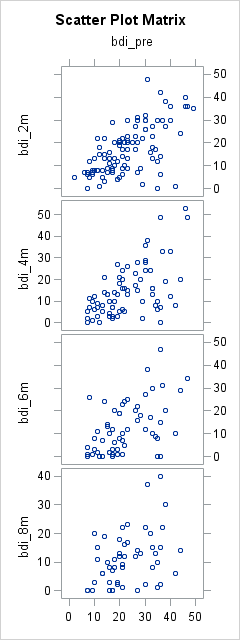
\includegraphics[width=0.9\textwidth]{L11_scatter.png}
\emp
\end{frame}


%===========================================================================================================================
\section[Output Delivery System]{Output Delivery System}
%===========================================================================================================================
\subsection{}
\begin{frame}
\tableofcontents[currentsection, hideallsubsections]
\end{frame}

\begin{frame}
\ft{Where graphs go}
\bi
\item By default our graphs so far have gone to the output window, or the results viewer
\item The \ttt{png's} automatically get saved as well - to find the location look for the path located in the lower right hand corner of your SAS window
\item Really, the Output Delivery System (ODS) determines where graphs go and what they look like
\ei
\end{frame}

\begin{frame}[fragile]
\frametitle{Output Delivery System}
The SAS Output Delivery System (ODS) can produce output in different \emph{destinations}.  The following work with ODS graphics:
\begin{enumerate}
    \item ODS LISTING
    \item ODS HTML
    \item ODS PDF
    \item ODF RTF
\end{enumerate}
\vskip10pt
\bmp{0.5\textwidth}
\emph{Styles} can be applied to the destinations to alter the general appearance. To view available styles:
\emp
\bmp{0.05\textwidth} \hspace{0.05in} \emp
\bmp{0.5\textwidth}
\footnotesize
\begin{code}{.0}
PROC TEMPLATE;
   LIST styles;
RUN;
\end{code}
\emp

\end{frame}
%
%\begin{frame}[fragile]
%\frametitle{ODS Styles}
%\begin{tabular}{|p{3cm} p{2.5cm}  p{4.5cm}|}
%\hline
%\ttb{ODS destination}  & \ttb{Default Style} & \ttb{Comments} \\
%\hline\hline
%LISTING & LISTING & White background, optimized for color format on white paper \\
%\hline
%HTML & HTMLBLUE & White background, optimized for HTML output \\
%\hline
%RTF & RTF & White background, colored fills\\
%\hline
%PDF & Printer & Optimized for PostScript and PDF output \\
%\hline
%\end{tabular}
%\vskip10pt
%
%\end{frame}
%
%\begin{frame}[fragile]
%\frametitle{Other commonly used styles}
%\begin{tabular}{|p{3cm} p{2.5cm}  p{4.5cm}|}
%\hline
%\ttb{Desired Output}  & \ttb{Style} & \ttb{Comments} \\
%\hline\hline
%Full color & DEFAULT & Gray background, optimized for HTML output \\
%\hline
%Fully color & ANALYSIS & Yellow background \\
%\hline
%Gray scale & JOURNAL & Interior filled areas are gray scale\\
%\hline
%Black and white & MONO-CHROME-PRINTER
% & Interior filled areas have no color \\
%\hline
%\end{tabular}
%\end{frame}
%
\begin{frame}[fragile]
\ft{Location of saved files}
To change the location of your saved png's, use \ttt{GPATH}.
\bmp{1.0\textwidth}
\footnotesize
\begin{code}{.0}
\textcolor{OrangeRed}{ODS HTML GPATH = "&dir" ;}
\textcolor{OrangeRed}{ODS GRAPHICS ON / IMAGENAME = "L11_scatter" RESET = INDEX ;}
PROC CORR DATA = flash.BtheB PLOTS = matrix ;
   VAR bdi_pre ;
   WITH bdi_2m bdi_4m bdi_6m bdi_8m ;
RUN ;
\end{code}
\emp
\end{frame}



\begin{frame}[fragile]
\frametitle{Default Destination}
The default destination for graphics output is the HTML destination, which is displayed in the Results Viewer window.  You can also specify the destination for your output.
\bmp{1.0\textwidth}
\footnotesize
\begin{code}{.0}
ODS destination FILE = "\emph{filename.ext}" STYLE=\emph{stylename};
  SAS/GRAPH (and/or other procedure) code to create a report
ODS destination CLOSE;
\end{code}
\emp
\end{frame}

\begin{frame}[fragile]
\frametitle{Example: change destination}
\bmp{1.05\textwidth}
\footnotesize
\begin{code}{.0}
\textcolor{OrangeRed}{ODS PDF FILE = "&dir.L11_correlation.pdf" STYLE = HTMLBlue ;}
\textcolor{OrangeRed}{OPTIONS NODATE NONUMBER ;}
PROC CORR DATA = flash.BtheB PLOTS = matrix ;
	VAR bdi_pre ;
	WITH bdi_2m bdi_4m bdi_6m bdi_8m ;
RUN ;
\textcolor{OrangeRed}{ODS PDF CLOSE ;}
\end{code}
\emp
\end{frame}







\end{document} 